%!TeX root=../tese.tex
%(dica para o editor de texto: este arquivo é parte de um documento maior)
% para saber mais: https://tex.stackexchange.com/q/78101/183146

\chapter{Redes neurais artificiais}
\label{cap:redes}

Neste capítulo são apresentados alguns conceitos básicos de \defi{aprendizado de máquina}, com foco nos algoritmos de redes neurais artificiais, em especial o \defi{perceptron}, que teve seu desenvolvimento inspirado nas redes neurais biológicas, ou seja, os neurônios e suas conexões no cérebro, conforme descrito por Kopec \citep{classic}.

Pode-se classificar as técnicas de aprendizado de várias formas, de acordo com alguma de suas características. Por exemplo, Géron \citep{hands} utiliza o grau de supervisão humana durante o seu funcionamento para classificá-los em aprendizado supervisionado ou não-supervisionado. Durante o aprendizado podem ou não ser fornecidos um conjunto de consultas e de respostas esperadas. Tais respostas foram dadas por humanos, ao menos neste momento, daí o termo ``supervisão humana''.

Neste texto os termos ``algoritmo'' e ``técnica'' serão usados livremente como sinônimos, pois uma técnica de aprendizado de máquina, no contexto atual, é um algoritmo executado no computador que tem por objetivo ajustar parâmetros de modelos estatísticos.

\section{Aprendizado de máquina supervisionado}

 Um algoritmo de \defi{aprendizado supervisionado} é usado quando conhecemos características dos dados que estamos utilizando. De modo geral já temos de antemão as respostas às consultas para os dados utilizados no treinamento. Por exemplo, se estamos classificando fotos de animais, possuímos um conjunto de fotos em que já sabemos quais são de gatos, cachorros, etc.

 O ato de rotular previamente os dados que usamos no treinamento é o que designamos de supervisão humana. Uma vez \emph{treinado}, o algoritmo recebe uma foto, ou seja, uma nova consulta e então fornece a resposta, neste caso se essa é a foto de um gato, ou cachorro, ou qualquer outra resposta dentre aquelas que foram dadas como exemplos durante o treinamento.

Dentro do aprendizado supervisionado temos duas técnicas principais. A primeira é a regressão, usada para prever valores, ou seja, fornecer respostas a consultas ainda inéditas, sejam dados do futuro ou valores de funções em pontos do domínio para os quais ainda não existem respostas. 

A segunda técnica é a classificação, usada para rotular ou dividir os dados em classes pré-determinadas, a partir de exemplos, que é exatamente o caso dos exemplos descritos nos parágrafos anteriores. Se as classes não são conhecidas deve-se utilizar um algoritmo de aprendizado não-supervisionado, descrito na próxima seção. 

Colocar exemplos...

\section{Aprendizado não-supervisionado}

Nesse tipo de aprendizado de máquina, não sabemos os rótulos dos dados que estamos lidando, assim o algoritmo poderá agrupar os dados de forma automática, por exemplo, se estivermos lidando com problemas de classificação. Aqui, as consultas podem ser coisas como ``quantos são os perfis dos clientes'' ou ``quantas espécies de flores existem nestas fotos'', e assim por diante.

Alguns métodos não-supervisionados de aprendizado foram enumeradas por Géron \citep{hands}. O \textbf{agrupamento} de dados similares sob uma inspiração geométrica. Nesse caso os dados são agrupados conforme suas posições num determinado espaço e utiliza-se algoritmos como $k$-vizinhos, $k$-means, $k$-medians, etc. Exemplos de aplicações são agrupamento de produtos em supermercados, interesses comuns de clientes em sites de conteúdo digital, etc.

Outra técnica é a \textbf{detecção de anomalias}, cujo objetivo é ter uma descrição de como os dados considerados ``normais'' se parecem, e usa-se esse agrupamento para detectar se novos dados estariam ``fora'' desse padrão. Um exemplo é a detecção de fraudes.

Também pode-se citar sobre a técnica de \textbf{estimação de densidades}, que tem como objetivo a estimação da função densidade de probabilidade de um conjunto de dados gerados por algum processo aleatório.

Colocar exemplos...

\section{Técnicas de classificação}

É uma das técnicas principais do aprendizado supervisionado, problemas desse tipo buscam aprender com um conjunto de dados previamente rotulados. Consultas do tipo ``a qual grupo pertence este cliente?'' ou ``que animal há nesta foto?'' podem ser modeladas por esses algoritmos. De modo geral, ele responde a consultas que dizem respeito às classes dos dados, e atribui para novos dados alguma classe que pertence ao conjunto de classes que usamos para rotular os dados iniciais.

Existem vários tipos de algoritmos de classificação, e dentre os descritos por Géron \citep{hands} citamos a máquina de vetor suporte (\eng{support vector machine}, SVM), árvores de decisão, florestas aleatórias que são um conjunto de muitas  árvores de decisão aleatoriamente definidas e, finalmente, as redes neurais artificiais.

Todas essas técnicas podem ser usadas para classificação linear ou não-linear, no sentido em que valores eles estão classificando, assim como na forma que está sendo feita essa classificação. Se visualizarmos os dados num espaço bidimensional, um algoritmo de classificação linear irá separar as classes de dados por retas, enquanto que um classificador não-linear poderá usar outra curva qualquer para a separação. 

Abstraindo o espaço bidimensional para os espaços multidimensionais dos dados que são comumente analisados, podemos pensar em hiperplanos, estruturas ($n{-}1$)-dimensionais de espaços $n$-dimensionais, para o caso dos classificadores lineares, ou subespaços quaisquer para os não-lineares.

Colocar exemplos de aplicações...

\section{A rede neural perceptron}

Uma rede neural artificial é um dentre vários métodos de classificação, ou seja, de aprendizado supervisionado, embora ela também possa ser usada para aplicaçõesd de aprendizado não supervisionado. De acordo com Kopec \citep{classic}, ele é utilizado como um classificador não-linear, e por isso pode ser utilizado para classificar ou prever quaisquer tipos de funções, que podem ou não ter uma relação linear com o tempo ou com qualquer outro domínio no qual estejam definidas.

Uma definição para uma rede neural artificial dada por Rosangela Ballini \citep{doutorado} é a de um sistema de processamento paralelo e distribuído baseado no sistema nervoso biológico, sendo compostos por elementos computacionais chamados neurônios, arranjados em padrões semelhantes às redes biológicas.

Na figura~\ref{fig:neuron} está uma representação de um neurônio biológico. Ele recebe impulsos elétricos de entrada através dos dentritos, que são transmitidos ou não através do núcleo, caso sejam ativados por ele, para os terminais de saída dos axônios. Os neurônios se comunicam através de sinapses, que são ligações entre os dentritos de um e os axônios de outro que realizam a transmissão dos sinais. 

\begin{figure}[htb]
\centering
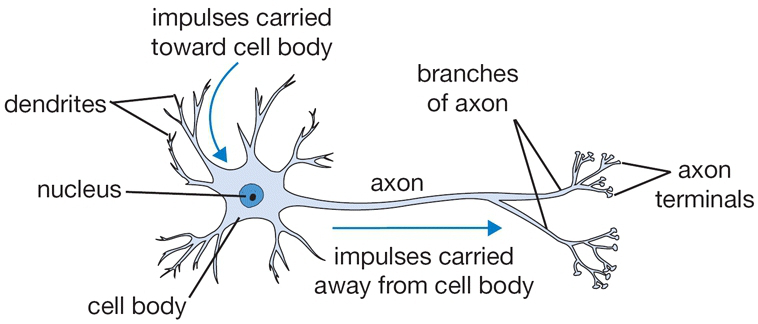
\includegraphics[width=8cm]{figuras/neuron}
\caption{Representação de um neurônio biológico.\footnote{Extraído de \url{https://cs231n.github.io/neural-networks-1/}}}
\label{fig:neuron}
\end{figure}

Dá-se o nome de \eng{perceptron} de camada única (\eng{single-layer perceptron}) ou simplesmente \eng{perceptron} a uma das primeiras e mais simples rede neural artificial a ser criada. Uma ilustração conceitual dela está na figura~\ref{fig:perceptron}. Mais recentemente foram criadas várias outras versões dessa rede, dentre as quais podemos citar o \eng{perceptron} de multi-camadas (\eng{multi-layer perceptron}). 

\begin{figure}[htb]
\centering
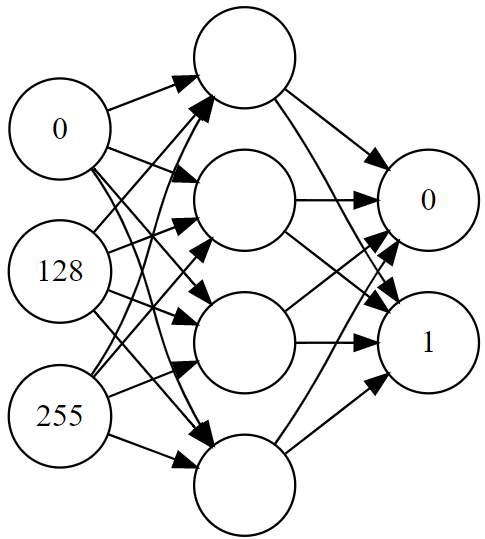
\includegraphics[width=5cm]{figuras/perceptron}
\caption{Rede neural simples, o perceptron de camada única.}
\label{fig:perceptron}
\end{figure}

Os neurônios são representados por círculos, dentro deles há um valor numérico que intuitivamente podemos atribuir ao nível ou grau de ativação do neurônio, mesmo que no caso biológico se restrinja aos valores $0$ e $1$, ou seja, ativados ou não. Cada coluna de neurônios representa uma camada, nesse caso, da esquerda para a direita temos a camada de entrada, a camada oculta e a camada de saída. As linhas representam as ligações entre os neurônios, sendo que cada neurônio de uma camada está ligado a todos da camada anterior.

O perceptron de camada única consiste de uma camada de neurônios de entrada, uma camada oculta de neurônios usados na otimização, e uma camada de saída, que irá conter os dados previstos, ou ainda as probabilidades do dado pertencer a alguma das classes que a rede poderá classificá-lo. E é o fato de haver uma camada oculta nesta rede que a define como sendo de ``camada única''. Caso houvessem mais do que uma camada oculta, ela seria do tipo ``multi-camadas'' mencionada acima.

De modo a entendermos as bases matemáticas do algoritmo, podemos começar de uma rede ainda mais básica, a partir um \eng{perceptron} que seja constituído de apenas $1$ neurônio na única camada oculta. Esta rede super simplificada, que está na figura~\ref{fig:neuronio}, pode ser útil para para o entendimento uma vez que neste caso será possível acompanhar graficamente o resultado da execução do algoritmo.

\begin{figure}[htb]
\centering
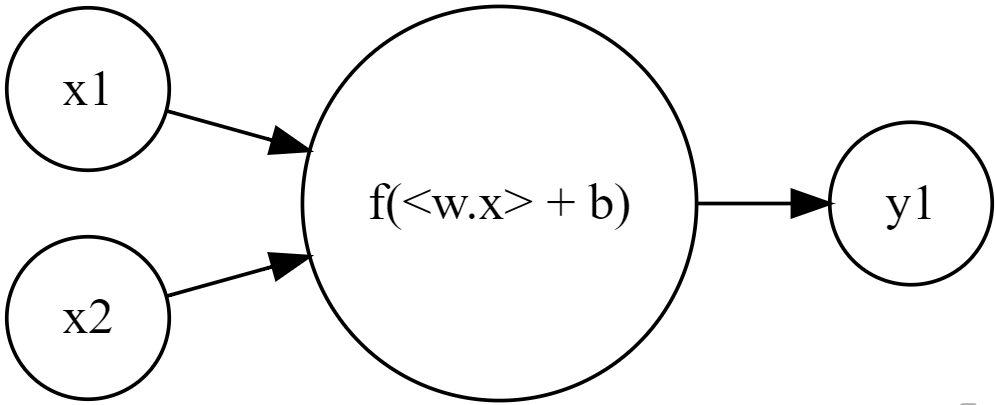
\includegraphics[width=8cm]{figuras/neuronio}
\caption{Rede neural mais simples ainda, apenas um neurônio oculto.}
\label{fig:neuronio}
\end{figure}

Esta rede possui $2$ neurônios na camada de entrada, que são os números reais $x_1$ e $x_2$, $1$ neurônio na camada oculta, no qual está a sua função de ativação $f(x_1w_1 + x_2w_2 + b)$, e $1$ neurônio na camada de saída, que neste caso é um número real $y_1$. Pode-se notar a semelhança dessa rede neural artificial com a sua inspiração biológica com a ajuda da figura~\ref{fig:neuron_model}. 

\begin{figure}[htb]
\centering
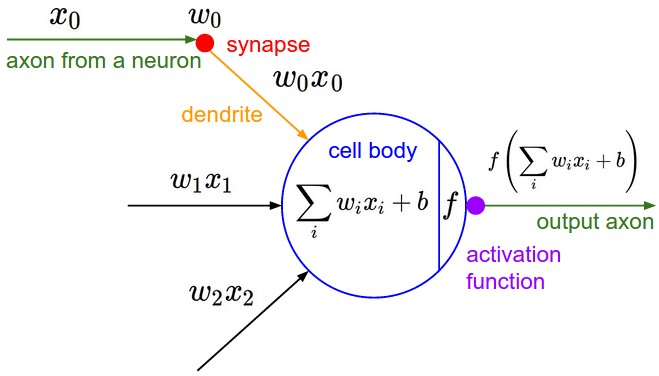
\includegraphics[width=8cm]{figuras/neuron_model}
\caption{Representação de um neurônio artificial.\footnote{Extraído de \url{https://cs231n.github.io/neural-networks-1/}}}
\label{fig:neuron_model}
\end{figure}

Temos os sinais de entrada (como o $x_1$) vindos como viriam os sinais dos axônios de outros neurônios. Eles entram pela camada de entrada da rede, ou dentritos do neurônio. A camada oculta processa as entradas com os pesos, definindo o formato final do sinal através de sua função de ativação, que aqui pode ser uma função real qualquer, mas com funcionalidade similar ao do núcleo do neurônio que ativa/transmite ou não o sinal recebido por ele. Por fim o sinal é enviado à camada de saída, ou aos axônios do neurônio, concluíndo o processamento.

A partir desta analogia podemos compreender o funcionamento básico da rede artificial \eng{perceptron}. Ela recebe uma lista de valores como entrada, que podemos representar por um vetor real $x$. O neurônio oculto representa uma transformação linear neste vetor, que podemos escrever como o produto escalar por um outro vetor real, o vetor de \defi{pesos} $w$, ou seja, $<w.x>$, que é o produto escalar usual dos números reais. A seguir, somamos um outro número real $b$ que é chamado de \defi{viés}, que possui o mesmo papel que a constante de interceptação da reta com o eixo vertical de um ajuste linear.

Por fim, é aplicada uma função de ativação não-linear sobre esta transformação, o que configura a saída deste neurônio: $f({<w.x>} + b)$, que é transmitida ao neurônio de saída, que pode aplicar uma transformação semelhante ou outra qualquer, dependendo da função de ativação utilizada em cada camada da rede. Por simplicidade mostramos uma rede bem simples, mas na prática podem haver muito mais camadas ocultas, e cada uma delas assim como a camada de saída, podem ter muitos neurônios cada.

Este processo de entrada, processamento e saída da rede é chamado de \defi{feedforward}, e consiste no nível mais fundamental do \eng{perceptron}. A partir daí, a forma como a rede será treinada, é o que define se ela será utilizada para um aprendizado supervisionado ou não-supervisionado.

Uma vez que estamos lidando com o aprendizado supervisionado, dever ser utilizado um algoritmo de treinamento que forneça à rede pares conhecidos de vetores de entradas e saídas esperadas, e um critério de avaliação de quão boa é a performance da rede para aproximar as suas saídas das saídas esperadas. 

Este critério é uma função que fornece uma medida da distância entre as saídas obtidas pela rede e as saídas esperadas, que é genericamente chamada de função de custo (\eng{cost function}). Se denotarmos por $y$ uma saída conhecida, e por $a^{(L)}$ uma saída obtida pela última camada, exemplos comumente usados são as normas usuais como a distância euclidiana ($(a^{(L)^2} + y^2)^{1/2}$), a função de erro absoluto ($|a^{(L)} - y|$), e a função de erro quadrático médio ($(a^{(L)} - y)^2$) , (\eng{mean square error}, MSE), que é a usada no algoritmo descrito por Kopec \citep{classic} e que será usado neste trabalho.

\section{Derivação matemática de um algoritmo de aprendizado}

Um dos algoritmos de treinamento que minimizam uma função de custo é o gradiente descendente (\eng{gradient descent}), que segundo Géron \citep{hands} é um algoritmo muito geral e que serve para encontrar soluções ótimas para uma grande variedade de problemas de otimização. A ideia geral é ajustar parâmetros iterativamente para otimizar a função de custo gradativamente.

O seu funcionamento utiliza a ideia fundamental do Cálculo em que utilizamos a derivada de uma função de forma a encontrar seus pontos extremos. Dada uma função $f{:}\mathbb{R}^n \rightarrow \mathbb{R}$, temos que se um ponto $x = \hat{x} \in \mathbb{R}$ é um ponto extremo de $f$ então é condição necessária\footnote{Mais detalhes em Guidorizzi \citep{guidorizzi2}. Um curso de cálculo Vol. 2, pág. 894.} que cada derivada parcial de primeira ordem de $f$ exista e seja igual a zero. Denotando $x = (x_0, x_1, \ldots, x_n)$ e $\hat{x} = (\hat{x_0}, \hat{x_1}, \ldots, \hat{x_n})$, temos:

\begin{equation}\label{grad_0}
\frac{\del f(\hat{x_0})}{\del x_0} = 0 ,\;\;\; \frac{\del f(\hat{x_1})}{\del x_1} = 0 ,\;\;\; \ldots ,\;\;\; \frac{\del f(\hat{x_n})}{\del x_n} = 0
\end{equation}

Usando a notação de vetores, podemos simplificar a equação acima, uma vez que o conjunto das derivadas parciais de uma função de várias variáveis é o vetor gradiente desta função, assim, denotando $\mathbf{0} \in \mathbb{R}^n = (0, 0, \ldots, 0)$, temos equivalentemente à equação \ref{grad_0}:

\begin{equation}\label{grad_1}
\nabla f(\hat{x}) = \mathbf{0}
\end{equation}
onde $\nabla{:}\mathbb{R}^n \rightarrow \mathbb{R}^n$ é a função que calcula o gradiente para um dado ponto de uma função.

Geometricamente é nos dada a intuição, por Luis Hamilton Guidorizzi \citep{guidorizzi2}, de que o vetor gradiente de um dado ponto de uma função nos dá a direção de maior aumento da função naquele ponto. Como nosso objetivo é minimizar a função de custo, fica explicado o nome do algoritmo como ``gradiente descendente'', de forma que devemos utilizar o sentido negativo do vetor gradiente.

Assim, podemos dizer que a direção de minimização da função está na direção do vetor gradiente, o que significa dar um passo ($f(x + dx)$) nessa direção no domínio da função, tal passo com tamanho que seja \emph{proporcional} a cada componente do vetor gradiente. Dessa forma podemos escrever $dx$ como sendo um passo na direção do mínimo da função de custo dessa forma:

\begin{equation}\label{grad_2}
dx = - \eta \nabla f(x)
\end{equation}
onde $\eta$ é a constante de proporcionalidade, que é conhecida como \defi{taxa de aprendizado}, que tem por objetivo tornar a velocidade do treinamento ajustável durante a execução do algoritmo, sendo tarefa do cientista de dados testar e obter os valores que dêem os melhores resultados caso-a-caso. 

Podemos observar as diferenças de utilizar uma taxa de aprendizado fixa ou variável (que mude a cada iteração do treinamento, por exemplo), utilizando gráficos. Suponha que estamos querendo minimizar uma função quadrática do tipo $f(x) = x^2$, essa restrição é particularmente útil uma vez que a função de custo que será utilizada, a MSE, é uma função quadrática deste tipo. Outra característica igualmente útil é que a segunda derivada deste tipo de função quadrática é sempre positiva\footnote{A segunda derivada de uma função de muitas variáveis é a matriz Hessiana, neste caso ela seria uma matriz definida positiva.}, o que implica que o ponto extremo encontrado será necessariamente um ponto de mínimo.

Inicialmente, sorteamos um ponto inicial e calculamos o valor da função e o valor do gradiente neste ponto. Se as componentes do gradiente não forem todas nulas (ou arbitrariamente próximas de zero), então quer dizer que não atingimos o mínimo, e dessa forma obtemos um novo ponto a partir deste somado com $dx$ definido acima na equação \ref{grad_2}. Repetimos este processo até que o gradiente do ponto atual seja arbitrariamente próximo do vetor nulo. Uma visualização deste processo, utilizando taxa de aprendizado fixada, está na Figura \ref{fig:grad_1}.

\begin{figure}[htb]
\centering
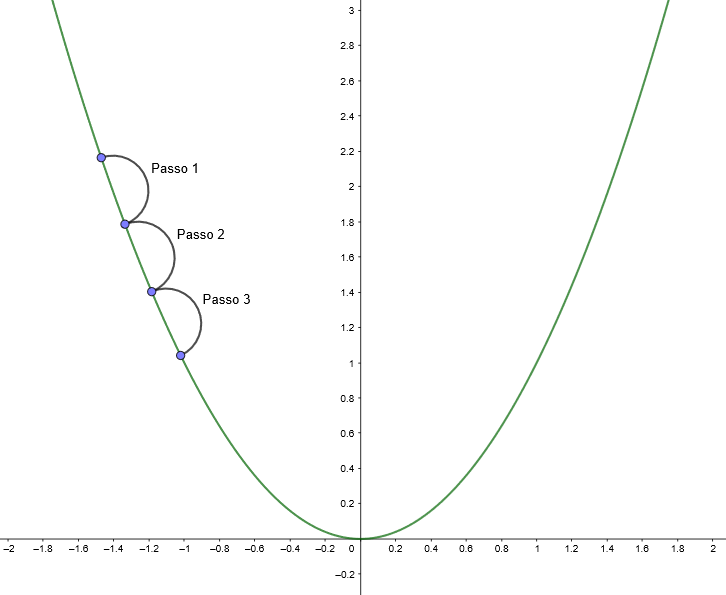
\includegraphics[height=8cm]{figuras/grad_1}
\caption{Visualização do método do gradiente descendente com taxa de aprendizado única. Os pontos azuis representam candidatos a ponto mínimo em cada iteração do algoritmo.}
\label{fig:grad_1}
\end{figure}

Podemos notar que as estimativas aproximam-se a uma velocidade constante do ponto de mínimo, que nesse caso ilustrativo é bem conhecido. Esse é o comportamento gerado por uma taxa de aprendizado fixa, e além disso com uma magnitude mediana. O que poderia acontecer se utilizarmos uma taxa de aprendizado muito grande é que com um passo do algoritmo, o ponto estimado poderia ir para o outro lado do arco da função, e depois retornar, e assim por diante, nunca convergindo para o mínimo, uma ilustração disso está na Figura \ref{fig:grad_2}.

\begin{figure}[htb]
\centering
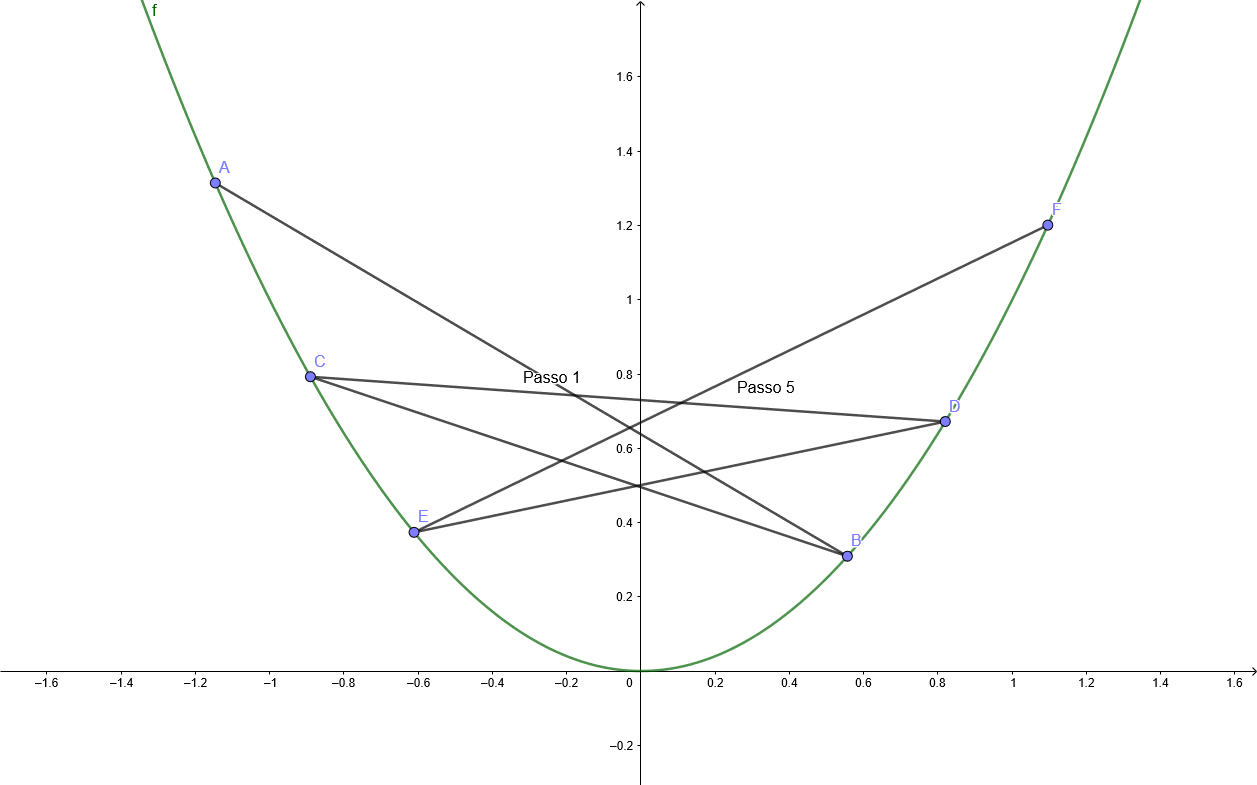
\includegraphics[height=8cm]{figuras/grad_2}
\caption{Visualização do método do gradiente descendente com taxa de aprendizado única. Ilustração do uso de um valor de taxa de aprendizado muito grande.}
\label{fig:grad_2}
\end{figure}

O caso oposto a este, ou seja, usar uma taxa muito pequena, claramente irá fazer com os passos dados sejam muito pequenos, e dessa forma o algoritmo demore muito a convergir, por isso é importante usar valores medianos que podem ser obtidos de forma heurística, embora na prática, conforme dito por Géron \citep{hands}, utiliza-se $\eta = 0.1$, sendo este um valor consensualmente utilizado pelo menos como ponto de partida.

A outra abordagem é utilizar valores variáveis, sendo o caso mais comum utilizar uma taxa que começa até mesmo maior do que o valor comum de $0.1$ mas que vai diminuindo a cada passo, numa tentativa de obter uma convergência mais rápida. Uma ilustração desse caso está na Figura \ref{fig:grad_3}.

\begin{figure}[htb]
\centering
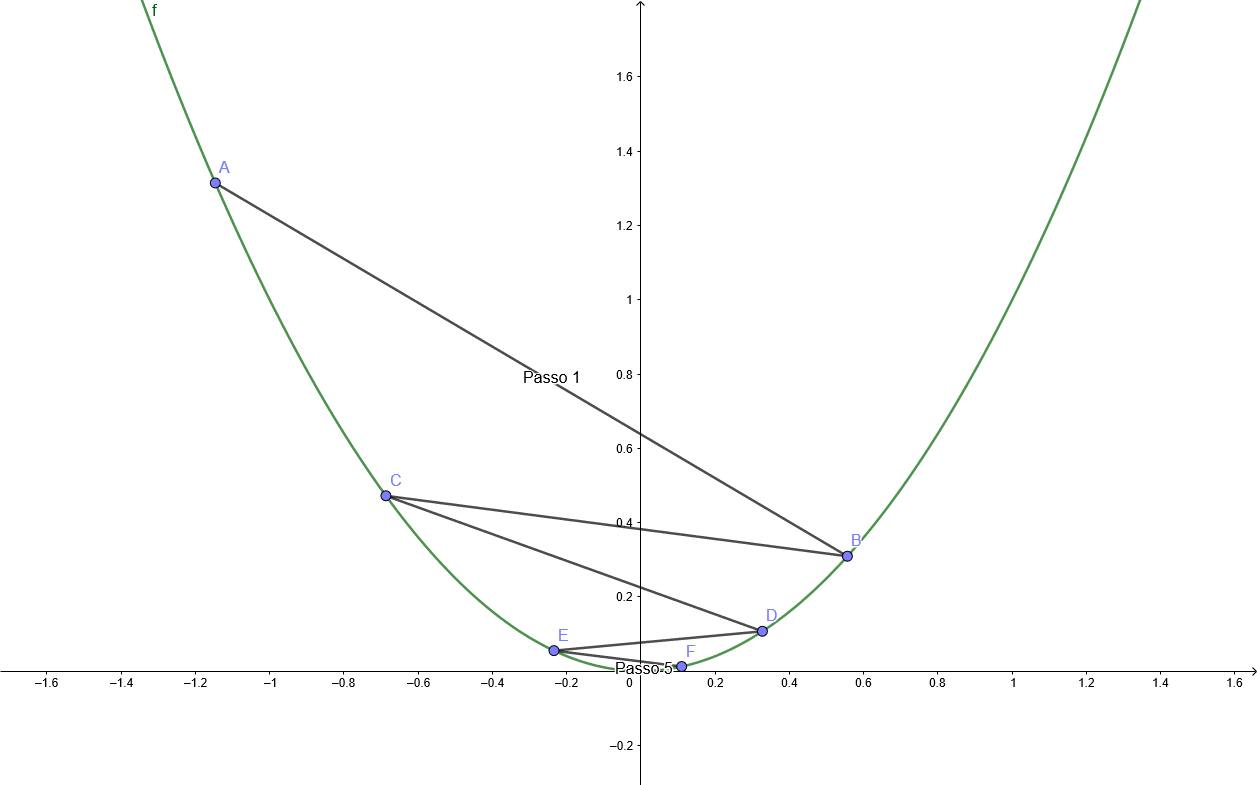
\includegraphics[height=8cm]{figuras/grad_3}
\caption{Visualização do método do gradiente descendente com taxa de aprendizado variável que vai diminuindo passo-a-passo do algoritmo.}
\label{fig:grad_3}
\end{figure}

Qualquer que seja o tipo de taxa de apredizado que venha a ser utilizado, permanece como melhor estratégia testar qual deles irá gerar o melhor resultado, a partir de algum problema com solução previamente conhecida, como a função $f(x) = x^2$, em que sabemos que o ponto de mínimo é atingido em $x = 0$, ou podemos testar em nosso problema-alvo, analisando diretamente os valores candidatos a mínimo obtidos pelo algoritmo como função do número do passo, criando assim outro tipo de gráfico, no qual não precisamos saber o formato da função objetivo, o que é razoável uma vez que não precisariamos de um método numérico para obter seu ponto de mínimo.

Podemos observar este comportamento genérico para os 4 casos acima mencionados, na Figura \ref{fig:grad_4} temos os gráficos de valores hipotéticos de candidatos a mínimo gerados por (a) taxa de aprendizado fixa e grande, (b) taxa de aprendizado fixa e pequena, (c) taxa de aprendizado fixa e mediana, (d) taxa de aprendizado decrescente.

\begin{figure}[htb]
\centering
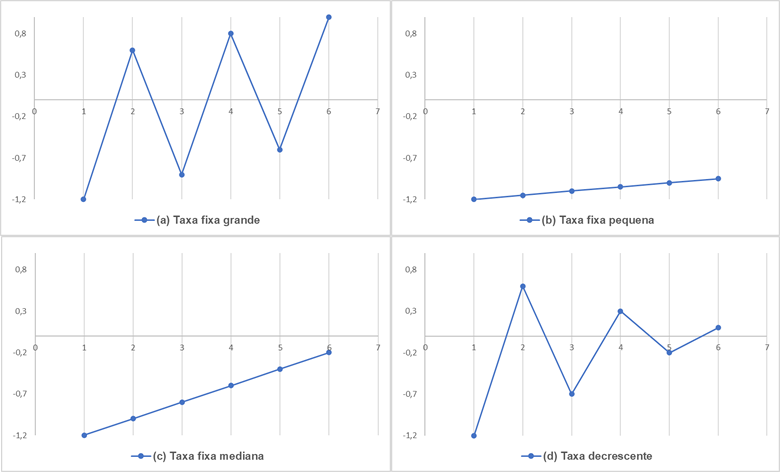
\includegraphics[width=14cm]{figuras/grad_4}
\caption{Comportamento de diferentes taxas de aprendizado nos valores candidatos a mínimo.}
\label{fig:grad_4}
\end{figure}

A partir deste comportamento geral, podemos testar nosso problema-alvo, verificar a qual comportamento ele mais se parece e assim decidir se devemos aumentar ou diminuir nossa taxa até obtermos um bom comportamento como aqueles vistos em (c) ou (d).

Colocar exemplos de outros algoritmos de otimização de função de custo...

